\chapter{面向微博的反讽识别}
\label{cha:exp_irony_det}

\section{本章引论}

社交媒体的发展对我们的语言体系带来了很大的影响,网络上出现了很多新颖的用词和句式,语言的表达方式越来越丰富,也越来越复杂。而反讽是在网络上常见的语言修饰手法之一, 这为反讽相关的研究带来了充足的数据基础。Henry Watson Fowler在《The King's English》一书中指出反讽的使用使得“表面意思和实际意思不同”。譬如一个人说“你这想法真有创意”,在字面意思上是对另一个人的赞同,但在特定背景下,如后接一句“你真相信这能实现吗”,那么发言者实际上可能暗示这个想法无法落地,表面上称赞为“有创意”,其实是指责这种想法不切实际。这在意图识别当中尤其重要,忽略反讽的使用会导致对内容的错误理解,而且这种理解是和真实意思截然相反的,因此识别出反讽的使用或许对相关的场景如情感识别、人机交互能起着正面的作用。

根据Joshi等人\cite{joshi2017automatic}对近年相关研究的总结,反讽识别可以大致分成基于规则的方法和基于机器学习的方法。基于规则的方法透过人工找出反讽中的语言规律,设计出对应的模式,然后在新样本中尝试识别出相应的模式出现。和机器学习方法对比,基于规则的方法优点在于无需模型训练,但要求研究员对反讽有充分的语言理解,设计的模式对样本的复盖程度决定了算法的识别能力。而随着近年深度学习快速发展,一些研究更专注于对词嵌入向量的使用以及人工神经网络的设计和选择。

国际比赛SemEval-2018的任务三\cite{van2018semeval}旨在促进英语微博中的反讽识别研究,其中包含了两个子任务。子任务一是二分类的反讽识别,需要识别微博是否有使用反讽。子任务二是四分类的反讽识别,是子任务一的拓展,除了判断微博是否包含反讽,反讽再细分成三个类别:基于相反语义的反讽 
、情景反讽、其他反讽。本章节中我们将基于SemEval-2018的任务三进行实验,采用比赛组织者提供的训练数据和测试数据,并透过和其他参赛系统进行比较来评估我们提出的框架的性能。

本章的内容安排如下。在章节\ref{sec:exp_irony_det_format}中,我们会基于章节\ref{sec:global_problem_analysis}首先给出当前问题的形式化表示。在章节\ref{sec:exp_irony_det_data}中我们再对具体实验数据进行观察,分析微博文本的特性以及各个反讽类别之间的不同。在章节\ref{sec:exp_irony_det_framework}中,我们会基于章节\ref{sec:global_framework}的框架给出我们对当前问题的系统框架。最后在章节\ref{sec:exp_irony_det_exp}给出实验的细节,以及对实验结果进行分析。

\section{形式化表示}
\label{sec:exp_irony_det_format}

在本章中,我们要研究单条微博的反讽类型识别。给定一个反讽类别集合$C$,对于一个微博集合$T$,对任意一条微博$t \in T$,它属于唯一一种情感类别$c \in C$。又给定一个词集合$V$,微博$t$经过文本预处理后可以表示为一个长度为$L$的词序列 $v = <v_1, v_2, ..., v_L>, v_i \in V, i \in [1, L]$。因为没有引入上下文信息,所以背景$B$在模型中忽略。那么我们的目标是找出一个映射关系$F_C$,使得$c=F_C(v)$。

\section{数据观察}
\label{sec:exp_irony_det_data}

我们的实验完全采用SemEval-2018的任务三比赛组织者提供的数据集,其中的语料收集自微博平台Twitter上发布于2014年至2015年之间的微博,再由人工标注得出每条微博的反讽类型。该比赛的两个子任务均采用了相同的戈语料但标注稍有不同。子任务一是二分类的反讽识别,需要识别微博是否有使用反讽,各类别的数据分布如表\ref{tab:semeval_2018_task3_A_data}所示,表\ref{tab:semeval_2018_task3_A_sample}为语料中两个类别的例子。可以看出没有反讽和带有反讽两个类别的样本在训练集上大致比例为1:1,在测试集上两个类别的分布大致为3:2。

\begin{table}[htb]
  \centering
  \begin{minipage}[t]{0.7\linewidth} % 如果想在表格中使用脚注,minipage是个不错的办法
  \caption{反讽识别子任务一各类别样本数量分布}
  \label{tab:semeval_2018_task3_A_data}
    \begin{tabularx}{\linewidth}{X|XX}
    \toprule[1.5pt]
    数据集 & 没有反讽 & 带有反讽 \\  
    \hline
    训练集 & 1923 & 1911 \\
    测试集 & 473  & 311 \\
    \bottomrule[1.5pt]
    \end{tabularx}
  \end{minipage}
\end{table}

\begin{table}[htb]
  \centering
  \begin{minipage}[t]{0.8\linewidth} % 如果想在表格中使用脚注,minipage是个不错的办法
  \caption{反讽识别子任务一样例}
  \label{tab:semeval_2018_task3_A_sample}
  \begin{tabularx}{\linewidth}{l|X}
    \toprule[1.5pt]
    反讽类别 & 例子 \\
    \hline
    没有反讽 & Had no sleep and have got school now \#not happy \\
    带有反讽 & I just love when you test my patience!! \#not \\
    \bottomrule[1.5pt]
  \end{tabularx}
  \end{minipage}
\end{table}

子任务二是四分类的反讽识别,是子任务一的拓展,除了判断微博是否包含反讽,反讽再细分成三个类别:基于相反语义的反讽、情景反讽、其他反讽。各类别的数据分布如表\ref{tab:semeval_2018_task3_B_data}所示,表\ref{tab:semeval_2018_task3_B_sample}为语料中各反讽类别的例子。可以看出带有反讽一类细分成三个子反讽类别后各个类别的分别变得明显的不均匀,三个子反讽类别中的样本数据量差异也较大,基于相反语义的言语反讽占了其中一半以上,在模型训练过程应有对应策略处理。

\begin{table}[htb]
  \centering
  \begin{minipage}[t]{\linewidth} % 如果想在表格中使用脚注,minipage是个不错的办法
  \caption{反讽识别子任务二各类别样本数量分布}
  \label{tab:semeval_2018_task3_B_data}
    \begin{tabularx}{\linewidth}{X|XXXX}
    \toprule[1.5pt]
    数据集 & 没有反讽 & 基于相反语义的反讽 & 情景反讽 & 其他反讽\\  
    \hline
    训练集 & 1923 & 1390 & 316  & 205 \\
    测试集 & 473  & 164  & 85  & 62 \\
    \bottomrule[1.5pt]
    \end{tabularx}
  \end{minipage}
\end{table}

\begin{table}[htb]
  \centering
  \begin{minipage}[t]{\linewidth} % 如果想在表格中使用脚注,minipage是个不错的办法
  \caption{反讽识别子任务二样例}
  \label{tab:semeval_2018_task3_B_sample}
  \begin{tabularx}{\linewidth}{l|X}
    \toprule[1.5pt]
    \small 反讽类别 & 例子 \\
    \hline
    \small 没有反讽 & Had no sleep and have got school now \#not happy \\
    \small 基于相反语义的反讽 & \small I really love this year’s summer; weeks and weeks of awful weather \\
    \small 情景反讽 & Most of us didn’t focus in the \#ADHD lecture. \#irony \\
    \small 其他反讽 & @someuser Yeah keeping cricket clean, that's what he wants \#Sarcasm \\
    \bottomrule[1.5pt]
  \end{tabularx}
  \end{minipage}
\end{table}

比赛组织者对四种反讽类别给出了对应的说明。对基于相反语义的反讽一类,文本中存在某部分内容表达了可评估的情感极性,但整条微博实际上表达了相反的情感极性。如表\ref{tab:semeval_2018_task3_B_sample}中的例子,“love”在字面意思上表达了正面的情感,但微博后半中“awful weather”提示实际情况引起了发言者的不适,发言者其实在表达对这个夏天坏天气的不满,这和“love”的正面情感恰恰相反。对于情景反讽一类,文本正描述某个场景,其中发生的事情和某种预期不符。如表\ref{tab:semeval_2018_task3_B_sample}中的例子,描述了一个参与讲座的场景,但“我们(us)”并没有专注于这场讲座,和“参与者应该专注于讲座内容”的预期相反。对于其他反讽一类,文本表达了讽刺的意思,但文本的字面意思和发言者表达的意思之间并不存在情感极性的反差。如表\ref{tab:semeval_2018_task3_B_sample}中的例子,发言者表示某人想要保持蟋蟀干净,字面上并不存在情感极性,但在句子后的井号标签提示了发言者表达了讽刺,认为“保持蟋蟀干净”是一样莫名奇妙的事情。最后是没有反讽一类,对于明显不可能包含反讽的文本,或者在背景信息不足的情况下不能确认其包含反讽的文本均属于这一类。

\subsection{文本长度}

我首先对数据集的文本经过简单分词后统计各个类别的样本中词数量的分布,以下简称为文本长度。表\ref{fig:semeval2018_task3_train_class_len}和表\ref{fig:semeval2018_task3_test_class_len}分别显示了训练集和测试集上各类别样本的文本长度。综合先见样本的文本长度不超过了50,样本的平均文本长度约为20个词。根据表\ref{fig:semeval2018_task3_train_class_len}我们可以看出“情景反讽”的样本整体的文本长度较其他类别的长,“没有反讽”和“基于相反语义的反讽”在文本长度分布上没有明显区别,“其他反讽”整体的文本长度则略高于前两者。再观察表\ref{fig:semeval2018_task3_test_class_len},同样地“没有反讽”和“基于相反语义的反讽”在文本长度分布上没有明显区别,“情景反讽”的文本长度略高于前两者,但不如训练集上明显。

\begin{figure}[H]
  \centering
  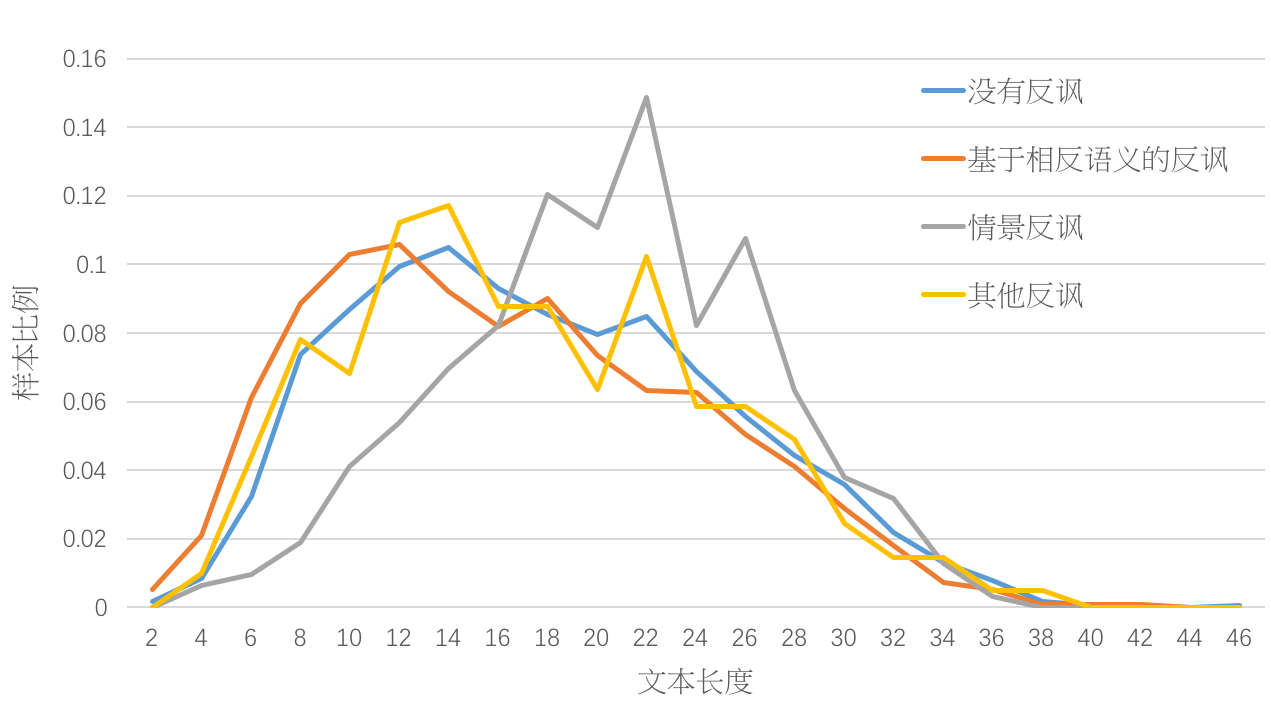
\includegraphics[width=\textwidth]{img/semeval2018_task3_train_class_len.png}
  \caption{反讽识别训练集上各类别文本长度分布}
  \label{fig:semeval2018_task3_train_class_len}
\end{figure}

\begin{figure}[H]
  \centering
  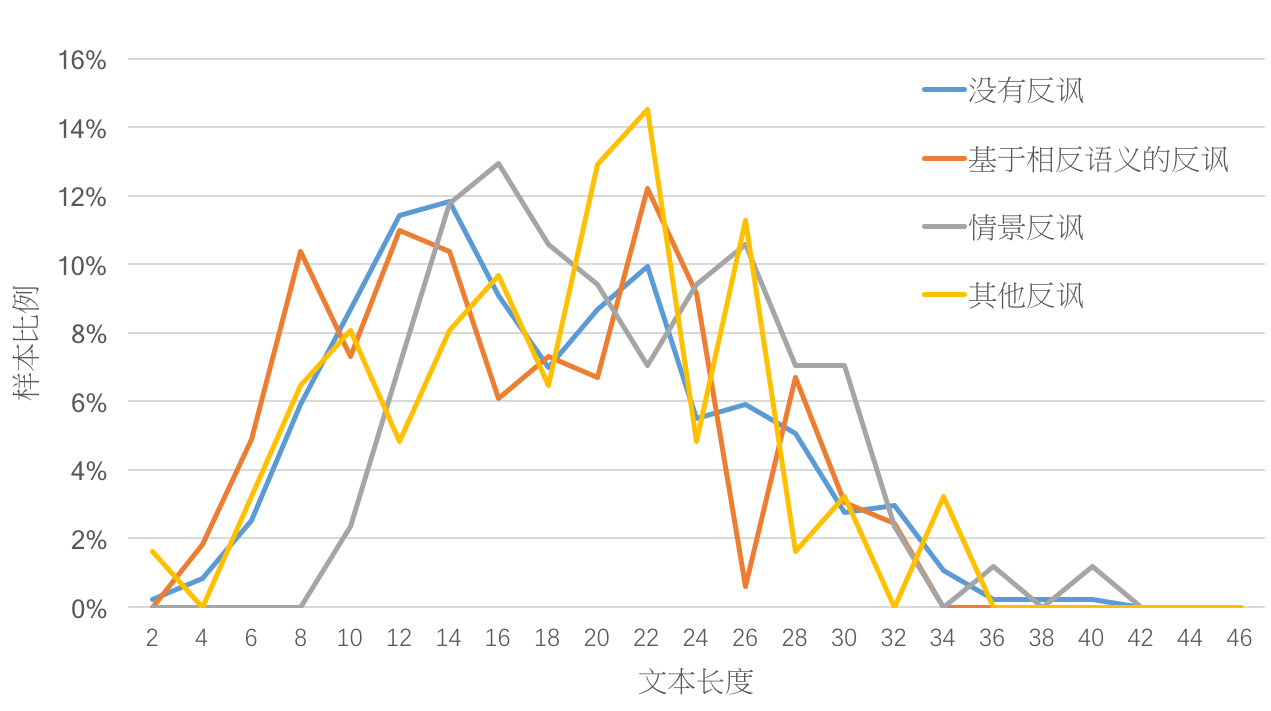
\includegraphics[width=\textwidth]{img/semeval2018_task3_test_class_len.png}
  \caption{反讽识别测试集上各类别文本长度分布}
  \label{fig:semeval2018_task3_test_class_len}
\end{figure}

\subsection{文本特征}

另外我们注意到语料中存在微博平台Twitter上特有的文本特征,出现频率较高的模式如下:

\begin{itemize}

\item 用户标签“@someuser”,对应微博上的一个用户,使用场景包括以下两种。一是作为句子中的名词使用,二是添加在句前或句末用于提示该用户的参与,不具有句法作用。

\item 井号标签“\#something”,使用场景大致分为以下两种。一是作为句子中的一部分,如“I \#do \#like \#it”,去除井号后满足正规的英语用法,此处以井号标签代替是对内容的强调。另一种是出现在句末,用于提示微博内容与标签对应内容相关,如句末出现“\#sarcasmtweet”明显表示讽刺。

\item 网站链接,在微博平台上支持附加一个网站链接以便,其中平台对链接进行了统一处理,在语料库中网站链接均形如“http://t.co/***”或“https://t.co/***”。

\item 转发标记“RT”(retweet),当用户转发某条微博并添加个人评论时,平台会自动在个人评论后附加转发的微博原文并以“RT”隔开。

\item 一些在社交媒体平台上常见的、有别于正规英语的用法,如拼写错误、缩略词、全大写字母的单词、表情符等,可以参考章节\ref{sec:text_preprocess}描述的例子。

\end{itemize}


\section{框架设计}
\label{sec:exp_irony_det_framework}

pass

\section{实验与分析}
\label{sec:exp_irony_det_exp}

pass

\subsection{数据预处理}

pass

\subsection{实验设置}

pass

\subsection{模型训练}

pass

\subsection{结果与分析}

pass

% \subsection{错误分析}

\section{本章小结}

pass

